\section{A known angle in the beam}\label{sec:knownangle}
\sectionstate{open}{R7; \texttt{sps\_beam\_test\_26/analysis/angled\_kernel} (geometry)}
\intent{A reference-free test: det4 rotated by 25.6\textdegree{} in the SPS beam. Hits and waveforms against the stage angle,
independent of the M3 telescope.}
\analysis{R7}{known-angle reconstruction, hits vs waveforms}
\begin{figure}[t]
  \centering
  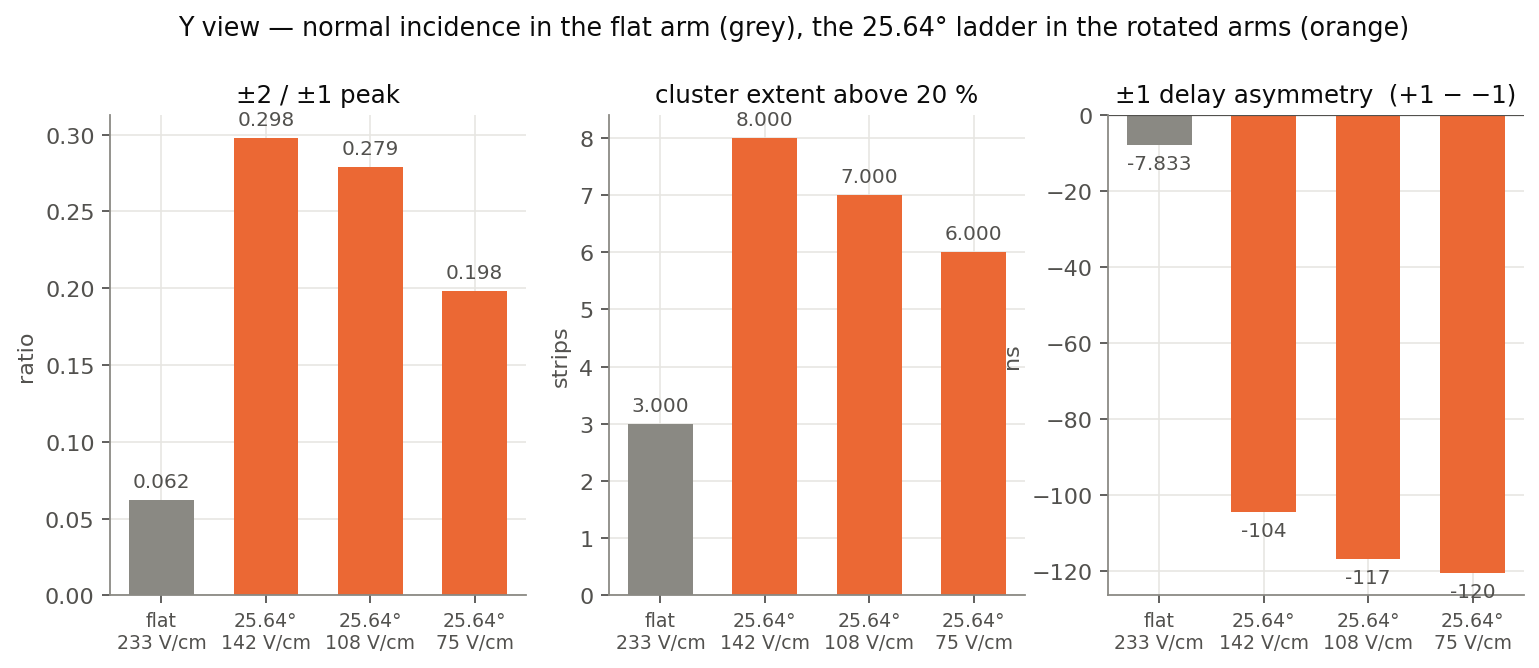
\includegraphics[width=0.6\linewidth]{known_angle_geometry}
  \caption{\tbw{det4 rotated in the beam.}}
  \label{fig:known_angle_geometry}
\end{figure}
\begin{figure}[t]
  \centering
  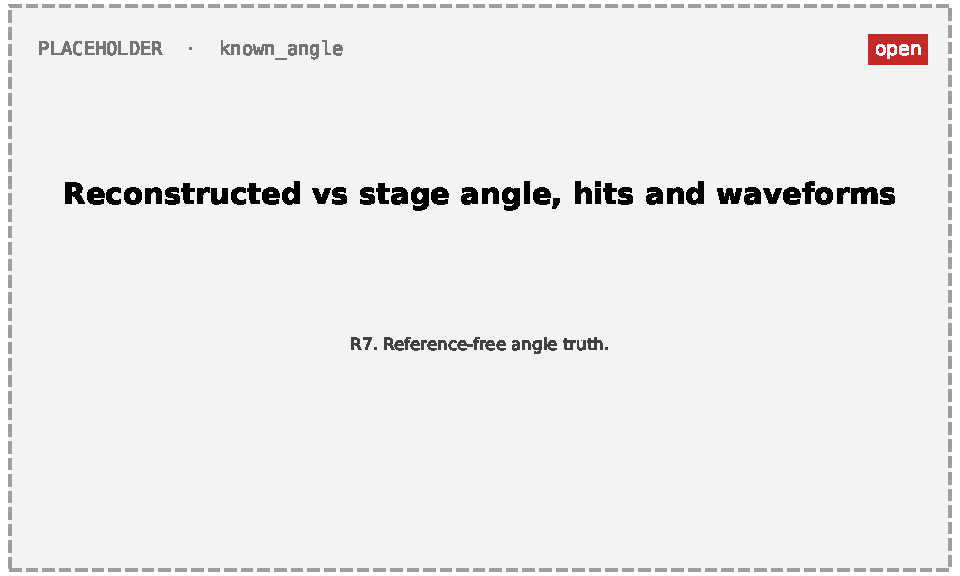
\includegraphics[width=0.7\linewidth]{known_angle}
  \caption{\tbw{Reconstructed angle against the stage angle.}}
  \label{fig:known_angle}
\end{figure}
